\documentclass[11pt, a4paper]{scrartcl}

% Core packages.
\usepackage[USenglish]{babel}
\usepackage[T1]{fontenc}
\usepackage[utf8]{inputenc}
\usepackage[top=1.5cm, left=1.5cm, right=1.5cm, bottom=2.5cm]{geometry}
% Math packages.
\usepackage{amssymb}
\usepackage{bbm}
\usepackage{bm}
\usepackage{cancel}
\usepackage{mathtools}
\usepackage{physics}
\usepackage{siunitx}
% Other packages.
\usepackage{csquotes}
\usepackage[hidelinks=true]{hyperref}
\usepackage{todonotes}
\usepackage{tikz}
\usepackage{xspace}
\usetikzlibrary{positioning}

% Document information.
\title{Pattern Recognition and Machine Learning}
\subtitle{Exercises}
\author{Fabian Damken}
\date{\today}

% Styling.
\MakeOuterQuote{"}
\mathtoolsset{showonlyrefs, showmanualtags}
\presetkeys{todonotes}{inline}{}

% Macros.
% Math.
\newcommand{\E}{\mathbb{E}}
\newcommand{\Var}{\mathbb{V}}
\DeclareMathOperator{\cov}{cov}
\newcommand{\KL}{D_\mathit{KL}}
\newcommand{\N}{\mathbb{N}}
\newcommand{\Z}{\mathbb{Z}}
\newcommand{\R}{\mathbb{R}}
\newcommand{\C}{\mathbb{C}}
\newcommand{\normal}{\mathcal{N}}
\newcommand{\transposed}{{\!\top\!}}
\renewcommand{\vec}[1]{\bm{#1}}
\newcommand{\mat}[1]{\bm{\mathrm{#1}}}
\newcommand{\given}{\,\vert\,}
\newcommand{\biggiven}{\,\big\vert\,}
\newcommand{\Biggiven}{\,\Big\vert\,}
\newcommand{\bigggiven}{\,\bigg\vert\,}
\newcommand{\Bigggiven}{\,\Bigg\vert\,}
\newcommand{\qed}{\hfill\(\square\)}
\newcommand{\eot}{\hfill\(\blacksquare\)}
\newcommand{\qedeot}{\hfill\(\square\blacksquare\)}
\newcommand{\liminmeansquare}{\mathop{\mathrm{l.i.m}}\displaylimits}
% Other.
\newcommand{\github}{\href{https://github.com/fdamken/gpml}{GitHub}\footnote{\url{https://github.com/fdamken/gpml}}\xspace}
\newcommand{\seegithub}{See \github.}
\newcommand{\task}[2]{\subsection*{Task #1: #2}}

\newcommand{\diffstar}{\texorpdfstring{\raisebox{-1pt}{\resizebox{!}{8pt}{\(\star\)}}}{*}}
\newcommand{\onestar}  {(\diffstar)}
\newcommand{\twostar}  {(\diffstar\,\diffstar)}
\newcommand{\threestar}{(\diffstar\,\diffstar\,\diffstar)}

\begin{document}
	\maketitle

	\begin{abstract}
		This document are my own results from working through the exercises of the book \emph{\@title} by Christopher M. Bishop. I tried to keep all notations as close to the book as possible. A \(\square\) marks the end of a proof while a \(\blacksquare\) marks the end of a task.
	\end{abstract}

	\section{Introduction}
		\subsection{Minimizing the Sum-of-Squares Error Function  \onestar}
			To find the optimal weights of the polynomial
			\begin{equation}
				y(x, \vec{w}) = \sum_{j = 0}^{M} w_j x^j  \label{eq:1-1-poly}
			\end{equation}
			with respect to the sum-of-squares error function
			\begin{equation}
				E(\vec{w}) = \frac{1}{2} \sum_{n = 1}^{N} \big( y(x_n, \vec{w}) - t_n \big)^2,  \label{eq:1-1-error}
			\end{equation}
			the derivative of the latter w.r.t. the weights \(\vec{w}\) has to be calculated. This requires the application of the chain rule. The partial derivatives of \eqref{eq:1-1-poly} are given as
			\begin{equation}
				\pdv{y(x, \vec{w})}{w_i} = \sum_{j = 0}^{M} \delta_{ij} x^j,
			\end{equation}
			where \( \delta_{ij} \) is the Kronecker delta. Combined with the partial derivative of \eqref{eq:1-1-error} w.r.t. the polynomial \eqref{eq:1-1-poly},
			\begin{equation}
				\pdv{E(\vec{w})}{y(x, \vec{w})} = \sum_{n = 1}^{N} \big( y(x_n, \vec{w}) - t_n \big),
			\end{equation}
			the whole derivative is given as
			\begin{align}
				\dv{E(\vec{w})}{w_i}
					&= \pdv{E(\vec{w})}{y(x, \vec{w})} \pdv{y(x, \vec{w})}{w_i}
					 = \sum_{n = 1}^{N} \sum_{j = 0}^{M} \delta_{ij} x^j \big( y(x_n, \vec{w}) - t_n \big)
					 = \sum_{n = 1}^{N} \sum_{j = 0}^{M} \delta_{ij} x^j \Bigg( \sum_{k = 0}^{M} w_k x_n^k - t_n \Bigg) \\
					&= \sum_{n = 1}^{N} \sum_{j = 0}^{M} \sum_{k = 0}^{M} \delta_{ij} w_k x_n^{j + k} - \sum_{n = 1}^{N} \sum_{j = 0}^{M} \delta_{ij} x_n^j t_n
					 = \sum_{n = 1}^{N} \sum_{k = 0}^{M} w_k x_n^{i + k} - \sum_{n = 1}^{N} x_n^i t_n \\
					&= \sum_{k = 0}^{M} w_k \underbrace{\sum_{n = 1}^{N} x_n^{i + k}}_{A_{ik} \,\coloneqq} - \underbrace{\sum_{n = 1}^{N} x_n^i t_n}_{T_i \,\coloneqq}
					 = \sum_{j = 0}^{M} A_{ik} w_k - T_i
			\end{align}
			Setting this quantity to zero yields exactly the linear equation system given in the task,
			\begin{equation}
				\sum_{j = 0}^{M} A_{ik} w_k = T_i,  \label{eq:1-1-linear}
			\end{equation}
			where \(A_{ik}\) and \(T_i\) are defined as in the above equation.

			\eot
		% end

		\subsection{Regularized Sum-of-Squares  \onestar}
			For the regularized error function
			\begin{equation}
				\tilde{E}(\vec{w}) = E(\vec{w}) + \frac{\lambda}{2} \lVert \vec{w} \rVert_2^2,
			\end{equation}
			the derivative is extended by the partial derivative of the regularization term,
			\begin{equation}
				\pdv{w_i} \frac{\lambda}{2} \lvert \vec{w} \rVert_2^2 = \lambda w_i.
			\end{equation}
			This yields the following derivative:
			\begin{equation}
				\dv{\tilde{E}(\vec{w})}{w_i}
					= \dv{E(\vec{w})}{\vec{w}} + \pdv{w_i} \frac{\lambda}{2} \lvert \vec{w} \rVert_2^2
					= \pdv{E(\vec{w})}{y(x, \vec{w})} \pdv{y(x, \vec{w})}{w_i} + \pdv{\lVert \vec{w} \rVert_2^2}{w_i}
					= \sum_{j = 0}^{M} A_{ik} w_k - T_i + \lambda w_i
			\end{equation}
			Analogous to \eqref{eq:1-1-linear}, the linear system of equations is given as
			\begin{equation}
				\sum_{j = 0}^{M} A_{ik} w_k = T_i - \lambda w_i
			\end{equation}
			which can be found by setting the derivative to zero. The variables \(A_{ik}\) and \(T_i\) are defined accordingly.

			\eot
		% end

		\subsection{Apples, Oranges, Limes, and Boxes  \twostar}
			Firstly, for each box \( B \in \{ r, b, g \} \), the probabilities of picking any fruit has to be calculated, i.e., the probabilities \( p(F \given B) \), where \( F \in \{ a, o, l \} \) is the random variable for the picked fruit with the possible values "apple", "orange", and "lime", respectively. The random variable \( R \) describes which fruit is removed. These probabilities depend on the box, too, and are given by the frequencies of the items in the boxes:
			\begin{center}
				\begin{tabular}{c|ccc}
					\( p(R \given B) \) & \(B = r\) & \(B = b\) & \(B = g\) \\ \hline
					     \(R = a\)      & \(3/10\)  &  \(1/2\)  & \(3/10\)  \\
					     \(R = o\)      &  \(2/5\)  &  \(1/2\)  & \(3/10\)  \\
					     \(R = l\)      & \(3/10\)  &   \(0\)   &  \(2/5\)
				\end{tabular}
			\end{center}
			The conditional probabilities \( p(F \given R, B) \) are then easy to calculate by subtracting one from the respective frequencies:
			\begin{center}
				\begin{tabular}{c|ccc}
					\( p(F \given R, B = r) \) & \(R = a\) & \(R = o\) & \(R = l\) \\ \hline
					        \(F = a\)          &  \(2/9\)  &  \(1/3\)  &  \(1/3\)  \\
					        \(F = o\)          &  \(4/9\)  &  \(1/3\)  &  \(4/9\)  \\
					        \(F = l\)          &  \(1/3\)  &  \(1/3\)  &  \(2/9\)
				\end{tabular}
				\qquad
				\begin{tabular}{c|ccc}
					\( p(F \given R, B = b) \) & \(R = a\) & \(R = o\) & \(R = l\) \\ \hline
					        \(F = a\)          &   \(0\)   &   \(1\)   &  \(1/2\)  \\
					        \(F = o\)          &   \(1\)   &   \(0\)   &  \(1/2\)  \\
					        \(F = l\)          &   \(0\)   &   \(0\)   &   \(0\)
				\end{tabular} \\
				\vspace{0.5cm}
				\begin{tabular}{c|ccc}
					\( p(F \given R, B = g) \) & \(R = a\) & \(R = o\) & \(R = l\) \\ \hline
					        \(F = a\)          &  \(2/9\)  &  \(1/3\)  &  \(1/3\)  \\
					        \(F = o\)          &  \(1/3\)  &  \(2/9\)  &  \(1/3\)  \\
					        \(F = l\)          &  \(4/9\)  &  \(4/9\)  &  \(1/3\)
				\end{tabular}
			\end{center}
			Of course, the probabilities \( p(F \given B, R = \text{None}) \), where no fruit is removes, is equivalent to \( p(R \given B) \) as each fruit is removed with equal probability. To get the probabilities \( p(F \given B) \), the joint probabilities
			\begin{equation}
				p(F, R \given B) = p(F \given R, B) \, p(R \given B)
			\end{equation}
			have to be calculated and marginalized:
			\begin{center}
				\begin{tabular}{c|ccc|c}
					\( p(F, R \given B = r) \) & \(R = a\) & \(R = o\) & \(R = l\) & \(p(F \given B = r)\) \\ \hline
					        \(F = a\)          & \(1/15\)  & \(2/15\)  & \(1/10\)  &       \(3/10\)        \\
					        \(F = o\)          & \(2/15\)  & \(2/15\)  & \(2/15\)  &        \(2/5\)        \\
					        \(F = l\)          & \(1/10\)  & \(2/15\)  & \(1/15\)  &       \(3/10\)        \\ \hline
					 \( p(R \given B = b) \)   & \(3/10\)  &  \(2/5\)  & \(3/10\)  &         \(1\)
				\end{tabular} \\
				\vspace{0.5cm}
				\begin{tabular}{c|ccc|c}
					\( p(F, R \given B = b \) & \(R = a\) & \(R = o\) & \(R = l\) & \(p(F \given B = b)\) \\ \hline
					        \(F = a\)         &   \(0\)   &  \(1/2\)  &   \(0\)   &        \(1/2\)        \\
					        \(F = o\)         &  \(1/2\)  &   \(0\)   &   \(0\)   &        \(1/2\)        \\
					        \(F = l\)         &   \(0\)   &   \(0\)   &   \(0\)   &         \(0\)         \\ \hline
					 \( p(R \given B = b) \)  &  \(1/2\)  &  \(1/2\)  &   \(0\)   &         \(1\)
				\end{tabular} \\
				\vspace{0.5cm}
				\begin{tabular}{c|ccc|c}
					\( p(F, R \given B = g \) & \(R = a\) & \(R = o\) & \(R = l\) & \(p(F \given B = g)\) \\ \hline
					        \(F = a\)         & \(1/15\)  & \(1/10\)  & \(2/15\)  &       \(3/10\)        \\
					        \(F = o\)         & \(1/10\)  & \(1/15\)  & \(2/15\)  &       \(3/10\)        \\
					        \(F = l\)         & \(2/15\)  & \(2/15\)  & \(2/15\)  &        \(2/5\)        \\ \hline
					 \( p(R \given B = g) \)  & \(3/10\)  & \(3/10\)  &  \(2/5\)  &         \(1\)
				\end{tabular}
			\end{center}
			The last column is the marginalization result and the last row is for validation as the probabilities should equal the ones given in the first table. Combined with the box probabilities
			\begin{align}
				p(B = r) &= 1/5 &
				p(B = b) &= 1/5 &
				p(B = g) &= 3/5
			\end{align}
			the joint probabilities
			\begin{equation}
				p(F, B) = p(F \given B) \, p(B)
			\end{equation}
			can be calculated as well as the interesting marginals \( p(F) \):
			\begin{center}
				\begin{tabular}{c|ccc|c}
					\( p(F, B) \) & \(B = r\) & \(B = b\) & \(B = g\) & \( p(F) \) \\ \hline
					  \(F = a\)   & \(3/50\)  & \(1/10\)  & \(9/50\)  & \(17/50\)  \\
					  \(F = o\)   & \(2/25\)  & \(1/10\)  & \(9/50\)  &  \(9/25\)  \\
					  \(F = l\)   & \(3/50\)  &   \(0\)   & \(6/25\)  &  \(3/10\)  \\ \hline
					 \( p(B) \)   &  \(1/5\)  &  \(1/5\)  &  \(3/5\)  &   \(1\)
				\end{tabular}
			\end{center}
			The last row is again for validation. To answer the first question in the task, the probability of picking an apple is
			\begin{equation}
				p(F = a) = 17/50 = 34\%.
			\end{equation}
			For computing the second question, the probability that a picked orange came from the green box, Bayes' theorem has to be invoked:
			\begin{equation}
				p(B = g \given F = o)
					= \frac{p(F = o \given B = g) \, p(B = g)}{p(F = o)}
					= \frac{3/10 \cdot 3/5}{9/25}
					= 1/2
					= 50\%.
			\end{equation}
			This concludes the task.

			\eot
		% end

		\subsection{Change of Variable  \twostar}
			Let \(\hat{x}\) and \(\hat{y}\) be the maxima of \(p_x(x)\) and \(p_y(y)\), respectively. Hence, the relations \( p_x'(\hat{x}) = 0 \) and \( p_y'(\hat{y}) = 0 \) hold. The derivative of \(p_y(y)\) w.r.t. \(y\) is given as
			\begin{equation}
				p_y'(y)
					= p_x'\big( g(y) \big) g'(y) \big\lvert g'(y) \big\rvert + p_x\big( g(y) \big) \dv{y} \big\lvert g'(y) \big\rvert.
			\end{equation}
			This derivative has to be zero for \(y = \hat{y}\):
			Assume \( \hat{x} = g(\hat{y}) \), then, as the derivative \( p_y'(y) \) has to be zero for \(y = \hat{y}\), the following must hold:
			\begin{align}
				0
					 = p_y'(\hat{y})
					&= p_x'\big( g(\hat{y}) \big) g'(\hat{y}) \big\lvert g'(\hat{y}) \big\rvert + p_x\big( g(\hat{y}) \big) \dv{y} \big\lvert g'(\hat{y}) \big\rvert \\
					&= \underbrace{p_x'(\hat{x})}_{=\, 0} g'(\hat{y}) \big\lvert g'(\hat{y}) \big\rvert + p_x(\hat{x}) \dv{y} \big\lvert g'(\hat{y}) \big\rvert \\
					&= p_x(\hat{x}) \dv{y} \big\lvert g'(\hat{y}) \big\rvert
			\end{align}
			But this only holds when \( \dv*{y} \big\lvert g'(\hat{y}) \big\rvert \) is zero\footnote{Since \(p_x(\hat{x})\) is the maximum of the probability density \(p_x(x)\) which must integrate to zero, it has to be greater than zero.}! Hence, the relation \( \hat{x} = g(\hat{y}) \) is not true in general.

			\qed

			As the second derivative of \(g\) vanishes for linear transformations, the relation \( \hat{x} = g(\hat{y}) \) holds if \(g\) is linear.

			\eot
		% end

		\subsection{Displacement Law  \onestar}
			From the definition of the variance,
			\begin{equation}
				\Var[f] = \E\Big[ \big( f(x) - \E[ f(x) ] \big)^2 \Big],
			\end{equation}
			and the linearity of the expectation operator, it follows that
			\begin{align}
				\Var[f]
					&= \E\Big[ \big( f(x) - \E[f(x)] \big)^2 \Big]
					 = \E\Big[ f^2(x) + \E^2[f(x)] - 2 f(x) \E[f(x)] \Big] \\
					&= \E\big[ f^2(x) \big] + \E^2[f(x)] - 2 \E^2[f(x)]
					 = \E\big[ f^2(x) \big] - \E^2[f(x)]
			\end{align}
			holds. This is the \emph{displacement law}.

			\qedeot
		% end

		\subsection{Covariance of Independent Variables  \onestar}
			\label{subsec:1-6}

			Let \(x\) and \(y\) be independent. Then \( p(x, y) = p(x) \, p(y) \) holds. Then the covariance
			\begin{equation}
				\cov[x, y] = \E_{x, y}[xy] - \E[x] \E[y]
			\end{equation}
			is zero as the expectation splits as \( \E_{x, y}[xy] = \E[x] \E[y] \). Let \(x\) and \(y\) be continuous, then
			\begin{equation}
				\E_{x, y}[xy]
					= \iint\! x y \underbrace{p(x, y)}_{\mathclap{=\, p(x) \, p(y)}} \dd{x} \dd{y}
					= \int\! x \, p(x) \dd{x} \int\! y \, p(y) \dd{y}
					= \Bigg(\! \int\! x \, p(x) \dd{x} \!\!\Bigg) \Bigg(\! \int\! y \, p(y) \dd{y} \!\!\Bigg)
					= \E[x] \E[y].
			\end{equation}
			Let \(x\) and \(y\) be discrete, then
			\begin{equation}
				\E_{x, y}[xy]
					= \sum_x \sum_y x y \, \underbrace{p(x, y)}_{\mathclap{=\, p(x) \, p(y)}}
					= \sum_x x \, p(x) \sum_y y \, p(y)
					= \Bigg(\! \sum_x x \, p(x) \!\Bigg) \Bigg(\! \sum_y y \, p(y) \!\Bigg)
					= \E[x] \E[y].
			\end{equation}
			For mixed cases, the relation \( \E_{x, y}[xy] = \E[x] \E[y] \) follows trivially. Hence, the covariance vanishes for two independent variables.

			\eot
		% end

		\subsection{Evaluation of Univariate Gaussian Integral  \twostar}
			To evaluate the squared Gaussian integral
			\begin{equation}
				I^2
					= \int_{-\infty}^{\infty} \int_{-\infty}^{\infty} \! \exp\bigg\{\! -\frac{1}{2 \sigma^2} x^2 - \frac{1}{2 \sigma^2} y^2 \bigg\} \dd{x} \dd{y}
					= \int_{-\infty}^{\infty} \int_{-\infty}^{\infty} \! \exp\bigg\{\! -\frac{1}{2 \sigma^2} \big( x^2 + y^2 \big) \bigg\} \dd{x} \dd{y},
			\end{equation}
			first a variable transformation from Cartesian to polar coordinates has to be transformed. As the radius \(r\) relates to the above integral by \( r^2 = x^2 + y^2 \) and the are element in polar coordinates is given as \( \dd A = r \dd{r} \dd{\varphi} \), the transformed integral is given as
			\begin{equation}
				I^2 = \int_{0}^{2\pi} \int_{0}^{\infty}\! \exp\bigg\{\! -\frac{r^2}{2 \sigma^2} \bigg\} r \dd{r} \dd{\varphi},
			\end{equation}
			where the integral bounds are changed to cover the whole space in polar coordinates. With the \(u\)-substitution \( u = r^2 \), \( \dd r = 1/(2 r) \dd{u} \), the integral evaluates to
			\begin{align}
				I^2
					&= \int_{0}^{2\pi} \int_{0}^{\infty}\! \exp\bigg\{\! -\frac{r^2}{2 \sigma^2} \bigg\} r \dd{r} \dd{\varphi}
					 = \frac{1}{2} \int_{0}^{2\pi} \int_{0}^{\infty}\! \exp\bigg\{\! -\frac{u}{2 \sigma^2} \bigg\} \dd{u} \dd{\varphi} \\
					&= \frac{1}{2} \int_{0}^{2\pi} \Bigg[ -\frac{1}{2 \sigma^2} \exp\bigg\{\! -\frac{u}{2 \sigma^2} \bigg\} \Bigg]_{u \,=\, 0}^{u \,\to\, \infty} \dd{\varphi}
					 = \sigma^2 \int_{0}^{2\pi} \Bigg[ 1 - \lim\limits_{u \,\to\, \infty} \exp\bigg\{\! -\frac{u}{2 \sigma^2} \bigg\} \Bigg] \dd{\varphi} \\
					&= \sigma^2 \int_{0}^{2\pi} \dd{\varphi}
					 = 2 \pi \sigma^2.
			\end{align}
			By taking the square-root on both sides, the result \( I = \sqrt{2 \pi \sigma^2} \) is obtained.

			This result can be used for showing that the Gaussian \( \normal(x \given \mu, \sigma^2) \) is normalized. Let \( \hat{x} = x - \mu \) such that \( \normal(x \given \mu, \sigma^2) = \normal(\hat{x} \given 0, \sigma^2) \)\footnote{This follows from the change of variables relation with \( \hat{x} = g(x) = x - \mu \) and \( g'(x) = 1 \).}. This eases the evaluation without loss of generality. Using this change of variables, the integral over the distribution can be evaluated:
			\begin{equation}
				\int_{-\infty}^{\infty}\! \normal(\hat{x} \given 0, \sigma^2) \dd{\hat{x}}
					= \int_{-\infty}^{\infty}\! \frac{1}{\sqrt{2 \pi \sigma^2}} \exp\bigg\{\! -\frac{\hat{x}^2}{2 \sigma^2} \bigg\} \dd{\hat{x}}
					= \frac{1}{\sqrt{2 \pi \sigma^2}} \underbrace{\int_{-\infty}^{\infty}\! \exp\bigg\{\! -\frac{\hat{x}^2}{2 \sigma^2} \bigg\} \dd{\hat{x}}}_{=\, \sqrt{2 \pi \sigma^2}} = 1
			\end{equation}
			This shows that the Gaussian is normalized.

			\eot
		% end

		\subsection{First and Second Moments of the Gaussian Distribution  \twostar}
			With the change of variables \( \hat{x} = x - \mu \), the integral evaluates as follows:
			\begin{align}
				\int_{-\infty}^{\infty}\! x \, \normal(x \given \mu, \sigma^2) \dd{x}
					&= \int_{-\infty}^{\infty}\! (\hat{x} + \mu) \, \normal(\hat{x} + \mu \given \mu, \sigma^2) \dd{\hat{x}} \\
					&= \underbrace{\int_{-\infty}^{\infty}\! \hat{x} \, \normal(\hat{x} + \mu \given \mu, \sigma^2) \dd{\hat{x}}}_{=\, 0} + \mu \underbrace{\int_{-\infty}^{\infty}\! \normal(\hat{x} + \mu \given \mu, \sigma^2) \dd{\hat{x}}}_{=\, 1}
					 = \mu
			\end{align}
			This equality to zero is due to the integrand being an odd function, thus the integral vanishes. Hence, the first moment is matched.

			\qed

			To derive the second moment of the Gaussian, the normalization constraint has to be differentiated. The derivative of \( \normal(x \given \mu, \sigma^2) \) w.r.t. the variance contains the following two components:
			\begin{align}
				\pdv{\sigma^2} \frac{1}{\sqrt{2 \pi \sigma^2}}
					&= -\frac{1}{\sqrt{8 \pi} \sigma^3} &
				\pdv{\sigma^2} \exp\bigg\{\! -\frac{(x - \mu)^2}{2 \sigma^2} \bigg\}
					&= \frac{(x - \mu)^2}{2 \sigma^4} \exp\bigg\{\! -\frac{(x - \mu)^2}{2 \sigma^2} \bigg\}
			\end{align}
			Plugging these into the whole derivative using the product rule yields
			\begin{align}
				\pdv{\sigma^2} \normal(x \given \mu, \sigma^2)
					&= -\frac{1}{\sqrt{8 \pi} \sigma^3} \exp\bigg\{\! -\frac{(x - \mu)^2}{2 \sigma^2} \bigg\}
					 + \frac{1}{\sqrt{2 \pi} \sigma} \frac{(x - \mu)^2}{2 \sigma^4} \exp\bigg\{\! -\frac{(x - \mu)^2}{2 \sigma^2} \bigg\} \\
					&= -\frac{1}{\sqrt{8 \pi} \sigma^3} \exp\bigg\{\! -\frac{(x - \mu)^2}{2 \sigma^2} \bigg\}
					 + \frac{(x - \mu)^2}{\sqrt{8 \pi} \sigma^5} \exp\bigg\{\! -\frac{(x - \mu)^2}{2 \sigma^2} \bigg\} \\
					&= -\frac{1}{\sqrt{8 \pi} \sigma^3} \exp\bigg\{\! -\frac{(x - \mu)^2}{2 \sigma^2} \bigg\}
					 + \frac{x^2 + \mu^2 - 2x\mu}{\sqrt{8 \pi} \sigma^5} \exp\bigg\{\! -\frac{(x - \mu)^2}{2 \sigma^2} \bigg\}.
			\end{align}
			Now this can be integrated separately by splitting the overall integral at the sums:
			\begin{gather}
				-\frac{1}{\sqrt{8 \pi} \sigma^3} \exp\bigg\{\! -\frac{(x - \mu)^2}{2 \sigma^2} \bigg\}
					= -\frac{1}{\sqrt{8 \pi} \sigma^3} \int_{-\infty}^{\infty}\! \exp\bigg\{\! -\frac{(x - \mu)^2}{2 \sigma^2} \bigg\} \dd{x}
					= -\frac{\sqrt{2 \pi} \sigma}{\sqrt{8 \pi} \sigma^3}
					= -\frac{1}{2 \sigma^2} \\
				\frac{1}{\sqrt{8 \pi} \sigma^5} \, x^2 \exp\bigg\{\! -\frac{(x - \mu)^2}{2 \sigma^2} \bigg\}
					= \frac{1}{\sqrt{8 \pi} \sigma^5} \int_{-\infty}^{\infty}\! x^2 \exp\bigg\{\! -\frac{(x - \mu)^2}{2 \sigma^2} \bigg\} \dd{x}
					= \frac{1}{2 \sigma^4} \int_{-\infty}^{\infty}\! x^2 \, \normal(x \given \mu, \sigma) \dd{x} \\
				\frac{\mu^2}{\sqrt{8 \pi} \sigma^5} \exp\bigg\{\! -\frac{(x - \mu)^2}{2 \sigma^2} \bigg\}
					= \frac{\mu^2}{\sqrt{8 \pi} \sigma^5} \int_{-\infty}^{\infty}\! \exp\bigg\{\! -\frac{(x - \mu)^2}{2 \sigma^2} \bigg\}
					= \frac{\sqrt{2 \pi} \sigma}{\sqrt{8 \pi} \sigma^5} \mu^2
					= \frac{1}{2 \sigma^4} \mu^2 \\
				-\frac{2\mu}{\sqrt{8 \pi} \sigma^5} \, x \exp\bigg\{\! -\frac{(x - \mu)^2}{2 \sigma^2} \bigg\}
					= -\frac{2\mu}{\sqrt{8 \pi} \sigma^5} \int_{-\infty}^{\infty}\! x \exp\bigg\{\! -\frac{(x - \mu)^2}{2 \sigma^2} \bigg\} \dd{x}
					= -\frac{2\sqrt{2 \pi} \sigma}{\sqrt{8 \pi} \sigma^5} \mu^2
					= -\frac{1}{\sigma^4} \mu^2
			\end{gather}
			Plugging everything together, the second moment of the Gaussian distribution is obtained:
			\begin{align}
				&&
				0 &= -\frac{1}{2 \sigma^2} + \frac{1}{2 \sigma^4} \int_{-\infty}^{\infty}\! x^2 \, \normal(x \given \mu, \sigma) \dd{x} + \frac{1}{2 \sigma^4} \mu^2 - \frac{1}{\sigma^4} \mu^2 & \\
				\iff &&
				\frac{1}{2 \sigma^4} \int_{-\infty}^{\infty}\! x^2 \, \normal(x \given \mu, \sigma) \dd{x} &= \frac{1}{2 \sigma^2} - \frac{1}{2 \sigma^4} \mu^2 + \frac{1}{\sigma^4} \mu^2 & \\
				\iff &&
				\int_{-\infty}^{\infty}\! x^2 \, \normal(x \given \mu, \sigma) \dd{x} &= \sigma^2 - \mu^2 + 2 \mu^2 = \sigma^2 + \mu^2 &
			\end{align}
			Hence, the second moment \( \E[x^2] \) is matched by the Gaussian.

			\qed

			With these first and second-order moments, it is trivial to show that \( \Var[x] = \sigma^2 \):
			\begin{equation}
				\Var[x] = \E[x^2] - \E^2[x] = \sigma^2 + \mu^2 - \mu^2 = \sigma^2
			\end{equation}
			This concludes all three elements of the task.

			\eot
		% end

		\subsection{Mode of the Gaussian Distribution  \onestar}
			Instead of maximizing the multivariate Gaussian distribution directly w.r.t. \(\vec{x}\), it is easier to maximize the log-probability because products are turned into sums and the exponential vanishes. This is valid because the logarithm is a strictly monotonic function. The log-Gaussian is given as
			\begin{equation}
				\log \normal(\vec{x} \given \vec{\mu}, \mat{\Sigma})
					= -\frac{D}{2} \log(2\pi) - \frac{1}{2} \log \lvert \mat{\Sigma} \rvert - \frac{1}{2} (\vec{x} - \vec{\mu})^\transposed \, \mat{\Sigma}^{-1} (\vec{x} - \vec{\mu}).
			\end{equation}
			Taking the derivative w.r.t. the mean \(\vec{\mu}\) lets the first two terms vanish as they are constant. The result derivative is then set to zero:
			\begin{equation}
				\pdv{\vec{\mu}} \log \normal(\vec{x} \given \vec{\mu}, \mat{\Sigma}) = \mat{\Sigma}^{-1} (\vec{x} - \vec{\mu}) \overset{!}{=} \vec{0}
				\qquad\implies\qquad
				\vec{x}_\mathrm{max} = \vec{\mu}
			\end{equation}
			This concluded the proof that the mean of the multivariate Gaussian is also its mode. The case for the univariate distribution follows as a corollary.

			\qedeot
		% end

		\subsection{Mean and Variance of Independent Random Variables  \onestar}
			Let \(x\) and \(z\) be independent (i.e., \( p(x, z) = p(x) \, p(z) \)). Then for the expectation is holds that
			\begin{align}
				\E[x + y]
					&= \iint\! (x + z) \, p(x, z) \dd{x} \dd{z}
					 = \iint\! (x + z) \, p(x) \, p(z) \dd{x} \dd{z} \\
					&= \iint\! x \, p(x) \, p(z) \dd{x} \dd{z} + \iint\! z \, p(x) \, p(z) \dd{x} \dd{z}
					 = \int\! x \, p(x) \dd{x} \underbrace{\int\! p(z) \dd{z}}_{=\, 1} + \int\! z \, p(z) \dd{z} \underbrace{\int\! p(x) \dd{x}}_{=\, 1} \\
					&= \int\! x \, p(x) \dd{x} + \int\! z \, p(z) \dd{z}
					 = \E[x] + \E[z].
			\end{align}
			For the variance, the proof is also straightforward:
			\begin{align}
				\Var[x + y]
					&= \E\Big[ \big( x + z - \E[x + z] \big)^2 \Big]
					 = \E\Big[ \big( x + z - \E[x] + \E[z] \big)^2 \Big]
					 = \E\Big[ \big( x + z - \E[x] - \E[z] \big)^2 \Big] \\
					&= \E\Big[ \E^2[x] + 2 \E[x] \E[z] + \E^2[z] - 2 \E[x] x - 2 \E[z] x + x^2 - 2 \E[x] z - 2 \E[z] z + 2 x z + z^2 \Big] \\
					&= \E^2[x] + 2 \E[x] \E[z] + \E^2[z] - 2 \E[x] \E[x] - 2 \E[z] \E[x] + \E[x^2] - 2 \E[x] \E[z] - 2 \E[z] \E[z] + 2 \E[xz] + \E[z^2] \\
					&= \E^2[x] + 2 \E[x] \E[z] + \E^2[z] - 2 \E^2[x] - 2 \E[x] \E[z] + \E[x^2] - 2 \E[x] \E[z] - 2 \E^2[z] + 2 \E[xz] + \E[z^2] \\
					&= -\E^2[x] - \E^2[z] + \E[x^2] - 2 \E[x] \E[z] + 2 \underbrace{\E[xz]}_{\mathclap{=\, \E[xz] = \E[x] \E[z]}} + \E[z^2] \\
					&= -\E^2[x] - \E^2[z] + \E[x^2] + \E[z^2]
					 = \Var[x] + \Var[z]
			\end{align}
			The equality \( \E[xz] = \E[x] \E[z] \) is true as \(x\) and \(z\) are independent (see \autoref{subsec:1-6} for the proof).

			\qedeot
		% end

		\subsection{Maximum Likelihood Estimates  \onestar}
			The log-likelihood is given as
			\begin{equation}
				\log p(X \given \mu, \sigma^2) = -\frac{N}{2} \log \sigma^2 - \frac{N}{2} \log(2\pi) - \frac{1}{2 \sigma^2} \sum_{n = 1}^{N} (x_n - \mu)^2.
			\end{equation}
			By taking the derivatives w.r.t. the mean and variance, the maximum likelihood estimates can be derived:
			\begin{gather}
				\pdv{\mu} \log p(X \given \mu, \sigma^2)
					= -\frac{1}{\sigma^2} \sum_{n = 1}^{N} (x_n - \mu)
					= -\frac{N}{\sigma^2} \mu - \frac{1}{\sigma^2} \sum_{n = 1}^{N}
					\overset{!}{=} 0
				\qquad\implies\qquad
				\mu_\mathrm{ML} = \frac{1}{N} \sum_{n = 1}^{N} x_n \\
				\pdv{\sigma^2} \log p(X \given \mu, \sigma^2)
					= -\frac{N}{2 \sigma^2} + \frac{1}{2 \sigma^4} \sum_{n = 1}^{N} (x_n - \mu)^2
					\overset{!}{0} 0
				\qquad\implies\qquad
				\sigma^2_\mathrm{ML} = \frac{1}{N} \sum_{n = 1}^{N} (x_n - \mu_\mathrm{ML})^2
			\end{gather}
			This concludes the derivation of the maximum likelihood estimators for the parameters of the univariate Gaussian distribution.

			\eot
		% end

		\subsection{Expectation of Maximum Likelihood Estimators  \twostar}
			If \(n \neq m\), the variables are independent and thus \( \E[x_n x_m] = \E[x_n] \E[x_m] = \mu^2 \). If \(n = m\), the variables are not independent and thus \( \E[x_n x_m] = \E[x_n^2] = \mu^2 + \sigma^2 \) which is the second moment. These results can be summarized using the Kronecker delta:
			\begin{equation}
				\E[x_n x_m] = \mu^2 + \delta_{nm} \sigma^2
			\end{equation}
			This result can now be used to derive the fact that the maximum likelihood estimator for the variance is biased:
			\begin{align}
				\E[\sigma^2_\mathrm{ML}]
					&= \E\Bigg[ \frac{1}{N} \sum_{n = 1}^{N} (x_n - \mu_\mathrm{ML})^2 \Bigg]
					 = \frac{1}{N} \sum_{n = 1}^{N} \E\Bigg[ \Bigg( x_n - \frac{1}{N} \sum_{m = 1}^{N} x_m \Bigg)^{\!\!2}\,\, \Bigg] \\
					&= \frac{1}{N} \sum_{n = 1}^{N} \E\Bigg[ x_n^2 + \frac{1}{N^2} \sum_{m = 1}^{N} \sum_{\ell = 1}^{N} x_m x_\ell - \frac{2}{N} \sum_{m = 1}^{N} x_n x_m \Bigg] \\
					&= \frac{1}{N} \sum_{n = 1}^{N} \Bigg( \E\big[x_n^2\big] + \frac{1}{N^2} \sum_{m = 1}^{N} \sum_{\ell = 1}^{N} \E[x_m x_\ell] - \frac{2}{N} \sum_{m = 1}^{N} \E[x_n x_m] \Bigg) \\
					&= \frac{1}{N} \sum_{n = 1}^{N} \Bigg( \mu^2 + \sigma^2 + \frac{1}{N^2} \sum_{m = 1}^{N} \sum_{\ell = 1}^{N} \big(\mu^2 + \delta_{m\ell} \sigma^2\big) - \frac{2}{N} \sum_{m = 1}^{N} \big(\mu^2 + \delta_{nm} \sigma^2\big) \Bigg) \\
					&= \frac{1}{N} \sum_{n = 1}^{N} \Big( \mu^2 + \sigma^2 + \mu^2 + \frac{1}{N} \sigma^2 - 2 \mu^2 - \frac{2}{N} \sigma^2 \Big) \\
					&= \frac{1}{N} \sum_{n = 1}^{N} \Big( \sigma^2 + \frac{1}{N} \sigma^2 - \frac{2}{N} \sigma^2 \Big)
					 = \frac{1}{N} \sum_{n = 1}^{N} \frac{N - 1}{N} \sigma^2
					 = \frac{N - 1}{N} \sigma^2
			\end{align}
			Similarly, it can be shown that the estimator for the mean is unbiased:
			\begin{equation}
				\E[\mu_\mathrm{ML}]
					= \E\Bigg[ \frac{1}{N} \sum_{n = 1}^{N} x_n \Bigg]
					= \frac{1}{N} \sum_{n = 1}^{N} \E[x_n]
					= \frac{1}{N} \sum_{n = 1}^{N} \mu
					= \mu
			\end{equation}
			Hence, the maximum likelihood estimator is not in general unbiased, but it can be.

			\eot
		% end

		\subsection{Expectation of Maximum Likelihood Variance Estimate  \onestar}
			Given the true mean \(\mu\) for estimating the variance, the variance estimator is unbiased:
			\begin{equation}
				\E[\sigma^2_\mathrm{ML}]
					= \E\Bigg[ \frac{1}{N} \sum_{n = 1}^{N} (x_n - \mu)^2 \Bigg]
					= \frac{1}{N} \sum_{n = 1}^{N} \E\Big[ (x_n - \mu)^2 \Big]
					= \frac{1}{N} \sum_{n = 1}^{N} \sigma^2
					= \sigma^2
			\end{equation}
			As shown in the previous task, this is not true if the maximum likelihood estimator is used for the mean

			\eot
		% end

		\subsection{Symmetric and Anti-Symmetric Matrices  \twostar}
			Let \(\mat{W}\) be an arbitrary square matrix. Then \( \mat{W} + \mat{W}^\transposed \) is symmetric and \( \mat{W} - \mat{W}^\transposed \) is anti-symmetric:
			\begin{gather}
				\big( \mat{W} + \mat{W}^\transposed\, \big)^\transposed
					= \mat{W}^\transposed + \mat{W}
					= \mat{W} + \mat{W}^\transposed \\
				\big( \mat{W} - \mat{W}^\transposed\, \big)^\transposed
					= \mat{W}^\transposed - \mat{W}
					= \big( \mat{W} - \mat{W}^\transposed \,\big)
			\end{gather}
			Hence, \(\mat{W}\) can be represented as the mean of the above matrices:
			\begin{equation}
				\frac{1}{2} \big( \mat{W}^S + \mat{W}^A \big)
					= \frac{1}{2} \big( \mat{W} + \mat{W}^\transposed + \mat{W} - \mat{W}^\transposed\, \big)
					= \frac{1}{2} \big( \mat{W} + \mat{W} \big)
					= \mat{W}.
			\end{equation}
			With \( \mat{W}^S = \big( \mat{W} + \mat{W}^\transposed\, \big) / 2 \) and \( \mat{W}^A = \big( \mat{W} - \mat{W}^\transposed\, \big) / 2 \), this concluded the proof that any matrix can be decomposed into a symmetric and an anti-symmetric matrix.

			\qed

			From this it follows directly that only the symmetric part of the coefficient matrix plays a role in higher-order polynomials. This is because the sum
			\begin{equation}
				\sum_{i = 1}^{D} \sum_{j = 1}^{D} w_{ij} x_i x_j
				=
				\sum_{i = 1}^{D} \sum_{j = 1}^{D} w_{ij}^S x_i x_j
				+
				\sum_{i = 1}^{D} \sum_{j = 1}^{D} w_{ij}^A x_i x_j
			\end{equation}
			splits into a symmetric and an anti-symmetric part. The anti-symmetric part vanished because for each element included in the sum, element mirrored across the diagonal is also included. Hence, as they have different signs, they cancel.

			The number of parameters in the coefficient matrix equals \( D (D + 1) / 2 \) because all elements above the diagonal equal the elements below the diagonal. Including the diagonal, the number of parameters thus is \( D + D - 1 + \cdots + 2 + 1 \) which equals \( D (D + 1) / 2 \) by the Gaussian summation rule.

			\eot
		% end

		\subsection{Number of Independent Parameters in M-th Order Term  \threestar}
			% TODO: 1.15 (***): Task: Number of parameters in polynomial.
		% end

		\subsection{Number of Independent Parameters in Multi-Dimensional Polynomial  \threestar}
			% TODO: 1.16 (***): Task: Number of parameters in polynomial.
		% end

		\subsection{Gamma Function  \twostar}
			By partially integrating the gamma function,
			\begin{equation}
				\Gamma(x)
					= \int_0^\infty\! u^{x - 1} e^{-u} \dd{u}
					= \frac{1}{x} \underbrace{\big[ u^x e^{-u} \big]_{u \,=\, 0}^{u \,\to\, \infty}}_{=\, 0} + \frac{1}{x} \underbrace{\int_0^\infty\! u^x e^{-u} \dd{u}}_{=\, \Gamma(x + 1)}
					= \frac{1}{x} \Gamma(x + 1)
				\quad\implies\quad
				\Gamma(x + 1) = x \Gamma(x),
			\end{equation}
			the result \( \Gamma(x + 1) = x \Gamma(x) \) can be obtained. The boundary terms vanish as \( 0^x e^{-0} = 0 \) and \( \lim\limits_{u \to \infty} u^x e^{-u} = 0 \). For the base case, \( \Gamma(1) \), the integral evaluates as
			\begin{equation}
				\Gamma(1)
					= \int_0^\infty\! u^{1 - 1} e^{-u} \dd{u}
					= \int_0^\infty\! e^{-u} \dd{u}
					= -\big[ e^{-u} \big]_{u \,=\, 0}^{u \,\to\, \infty}
					= 1.
			\end{equation}
			Hence, for integers \(n\), \( \Gamma(n + 1) = n! \).

			\qedeot
		% end

		\subsection{Surface Area and Volume of a \(D\)-Dimensional Unit Hypersphere  \twostar}
			The integral on the right hand side can be transformed using a \(u\)-substitution with \( u = r^2 \) after introducing a square and a square-root in the first term:
			\begin{align}
				\int_0^\infty\! r^{D - 1} e^{-r^2} \dd{r}
					= \int_0^\infty\! \big(r^2\big)^{(D - 1) / 2} e^{-r^2} \dd{r}
					= \frac{1}{2} \int_0^\infty\! u^{-1/2} u^{(D - 1) / 2} e^{-u} \dd{u}
					= \frac{1}{2} \int_0^\infty\! u^{D/2 - 1} e^{-u} \dd{u}
					= \frac{1}{2} \, \Gamma(D / 2)
			\end{align}
			It remains to evaluate the left hand integral(s). The value of these can be obtained by setting \( \sigma^2 = 1/2 \) in the Gaussian integral \( I = \int_{-\infty}^{\infty}\! e^{-x^2 / (2 \sigma^2)} \dd{x} \):
			\begin{equation}
				\int_{-\infty}^{\infty}\! e^{-x_i^2} \dd{x_i}
					= \sqrt{2 \pi \sigma^2}
					\overset{\;\sigma^2 \,=\, 1/2}{=} \sqrt{\pi}
			\end{equation}
			Plugging these two results into the equation yields the desired results:
			\begin{equation}
				\prod_{i = 1}^{D} \int_{-\infty}^{\infty}\! e^{-x_i^2} \dd{x_i} = S_D \int_0^\infty\! r^{D - 1} e^{-r^2} \dd{r}
				\quad\iff\quad
				\prod_{i = 1}^{D} \sqrt{\pi} = S_D \frac{1}{2} \, \Gamma(D / 2)
				\quad\iff\quad
				S_D = \frac{2 \pi^{D/2}}{\Gamma(D / 2)}
			\end{equation}
			Hence, the surface area of a \(D\)-dimensional sphere is given as \( S_D = \flatfrac{2 \pi^{D/2}}{\Gamma(D / 2)} \). Using this result, the formula for the volume
			\begin{equation}
				V_D = S_D \int_0^1\! r^{D - 1} \dd{r} = \frac{S_D}{D} \big[ r^D \big]_{r \,=\, 0}^{r \,=\, 1} = \frac{S_D}{D}
			\end{equation}
			in \(D\) dimensions can also directly be obtained.

			\qed

			For \(D = 2\) and \(D = 3\), the formulas reduce to
			\begin{align}
				S_2 &= \frac{2 \pi^{2/2}}{\Gamma(2 / 2)} = 2 \pi &
				V_2 &= \frac{S_2}{2} = \pi &
				S_3 &= \frac{2 \pi^{3/2}}{\Gamma(3 / 2)} = \frac{2 \pi^{3/2}}{\pi^{1/2} / 2} = 4 \pi^2 &
				V_3 &= \frac{S_3}{3} = \frac{4}{3} \pi^2
			\end{align}
			which equal the commonly known formulas for the surface area and volume of a circle and sphere.

			\eot
		% end

		\subsection{Volume Ratio of \(D\)-Dimensional Hypersphere and -cube  \twostar}
			The volume of a \(D\)-dimensional hypercube with side length \(2a\) is given as \((2a)^D\). For a unit hypercube, \(a = 1\), this reduces to \(2^D\). Hence, with the results from the first task, the ratio between the volume of a \(D\)-dimensional hypersphere and a \(D\)-dimensional hypercube is given as
			\begin{equation}
				\frac{\text{Volume of Sphere}}{\text{Volume of Cube}}
					= \frac{\frac{2 \pi^{D/2}}{D \, \Gamma(D / 2)}}{2^D}
					= \frac{2 \pi^{D/2}}{2^D D \, \Gamma(D / 2)}
					= \frac{\pi^{D/2}}{2^{D - 1} D \, \Gamma(D / 2)}.
			\end{equation}

			To make the subsequent derivations easier, let \( \tilde{D} = D/2 - 1 \) such that \( \Gamma(D/2) = \Gamma(\tilde{D} + 1) \) with the inverse transformation \( D = 2 (\tilde{D} + 1) \). The above ratio then---in terms of \(\tilde{D}\)---is
			\begin{equation}
				\frac{\pi^{D/2}}{2^{D - 1} D \, \Gamma(D / 2)}
					= \frac{1}{2} \frac{\pi^{\tilde{D}}}{2^{2 \tilde{D}} 2 (\tilde{D} + 1) \, \Gamma(\tilde{D} + 1)}.
			\end{equation}
			By replacing the gamma function with the Sterling approximation
			\begin{equation}
				\Gamma(\tilde{D} + 1) \approx (2\pi)^{1/2} e^{-\tilde{D}} \tilde{D}^{\tilde{D} + 1/2},
			\end{equation}
			an upper bound on the ratio can be found:
			\begin{align}
				\frac{\pi^{\tilde{D}}}{2^{2 \tilde{D} + 1} 2 (\tilde{D} + 1) \, \Gamma(\tilde{D} + 1)}
					&= \frac{1}{2} \frac{\pi^{\tilde{D}}}{2^{2 \tilde{D}} 2 (\tilde{D} + 1) (2\pi)^{1/2} e^{-\tilde{D}} \tilde{D}^{\tilde{D} + 1/2}}
					 = \frac{1}{2} \frac{\pi^{\tilde{D}}}{2^{2 \tilde{D}} 2 (\tilde{D} + 1) 2^{1/2} \pi^{1/2} e^{-\tilde{D}} \tilde{D}^{\tilde{D} + 1/2}} \\
					&= \frac{1}{2^{5/2}} \frac{\pi^{\tilde{D} - 1/2} e^{\tilde{D}}}{2^{2 \tilde{D}} (\tilde{D} + 1) \tilde{D}^{\tilde{D} + 1/2}}
					 \leq \frac{1}{2^{5/2}} \frac{\pi^{\tilde{D} - 1/2} e^{\tilde{D}}}{2^{2 \tilde{D}} (1 + 1) \tilde{D}^{\tilde{D} + 1/2}}
					 = \frac{1}{2^{9/2}} \frac{\pi^{\tilde{D} - 1/2} e^{\tilde{D}}}{2^{2 \tilde{D}} \tilde{D}^{\tilde{D} + 3/2}} \\
					&\leq \frac{1}{2^{9/2}} \frac{4^{\tilde{D} - 1/2} 4^{\tilde{D}}}{2^{2 \tilde{D}} \tilde{D}^{\tilde{D} + 1/2}}
					 = \frac{1}{2^{9/2}} \frac{4^{-1/2} 4^{2\tilde{D}}}{4^{\tilde{D}} \tilde{D}^{\tilde{D} + 1/2}}
					 = \frac{1}{2^{11/2}} \frac{4^{\tilde{D}}}{\tilde{D}^{\tilde{D} + 1/2}}
					 \overset{\tilde{D} \,\to\, \infty}{\to} 0
			\end{align}
			It is easy to see that this upper bound converges to zero as \( \tilde{D} \to \infty \) (implying \( D = 2 (\tilde{D} + 1) \to \infty \)). As also every element if the series is positive, the ratio vanishes in the limit by the squeeze theorem.

			\qed

			The distance from the center of the hypercube to one of the corners is given as
			\begin{equation}
				d_c = \sqrt{\sum_{i = 1}^{D} a^2} = \sqrt{D a^2} = a \sqrt{D}
			\end{equation}
			by the Pythagorean theorem. The perpendicular distance to one of the sides is given as \(d_p = a\), which follows directly from the definition of the concentric hypercube. Thus, the respective ratio is \( d_c/d_p = \sqrt{D} \) which is independent from the size of the cube.

			\eot
		% end

		\subsection{Gaussian Distribution in High Dimensions  \twostar}
			% TODO: 1.20 (**): Task: Gaussian in High Dimensions
		% end

		\subsection{Upper Bound on the Misclassification Probability  \twostar}
			Let \( a, b \in \R \) such that \( b \geq a \geq 0 \). Then \( a^2 = a^2 \geq ab \)
			Let \( a, b, c \in \R \) such that \( 0 \leq a \leq b \) and \( b = a + c \). Then \( ab = a (a + c) = a^2 + ac \geq a^2 \). Hence, \( a \leq \sqrt{ab} \).
			\qed

			Let \( \mathcal{R} \coloneqq \mathcal{R}_1 \cup \mathcal{R}_2 \) where \(\mathcal{R}_1\) and \(\mathcal{R}_2\) are disjoint. Then an upper bound on the misclassification probability can be found by adding, subtracting, and discarding the probability of being correct:
			\begin{align}
				p(\mathrm{mistake})
					&= \int_{\mathcal{R}_1}\! p(\vec{x}, \mathcal{C}_2) \dd{\vec{x}} + \!\int_{\mathcal{R}_2}\! p(\vec{x}, \mathcal{C}_1) \dd{\vec{x}} \\
					&= \int_{\mathcal{R}_1}\! p(\vec{x}, \mathcal{C}_2) \dd{\vec{x}} + \!\int_{\mathcal{R}_2}\! p(\vec{x}, \mathcal{C}_1) \dd{\vec{x}}
						\begin{aligned}[t]
							 + \!\int_{\mathcal{R}_1}\! p(\vec{x}, \mathcal{C}_1) \dd{\vec{x}} + \!\int_{\mathcal{R}_2}\! p(\vec{x}, \mathcal{C}_2) \dd{\vec{x}} \\
							 - \!\int_{\mathcal{R}_1}\! p(\vec{x}, \mathcal{C}_1) \dd{\vec{x}} - \!\int_{\mathcal{R}_2}\! p(\vec{x}, \mathcal{C}_2) \dd{\vec{x}}
						\end{aligned} \\
					&= \int_{\mathcal{R}_1}\! \big( p(\vec{x}, \mathcal{C}_1) + p(\vec{x}, \mathcal{C}_2) \big) \dd{\vec{x}} + \!\int_{\mathcal{R}_2}\! \big( p(\vec{x}, \mathcal{C}_1) + p(\vec{x}, \mathcal{C}_2) \big) \dd{\vec{x}}
						- \!\int_{\mathcal{R}_1}\! p(\vec{x}, \mathcal{C}_1) \dd{\vec{x}} - \!\int_{\mathcal{R}_2}\! p(\vec{x}, \mathcal{C}_2) \dd{\vec{x}} \\
					&\leq \int_{\mathcal{R}_1}\! \big( p(\vec{x}, \mathcal{C}_1) + p(\vec{x}, \mathcal{C}_2) \big) \dd{\vec{x}} + \!\int_{\mathcal{R}_2}\! \big( p(\vec{x}, \mathcal{C}_1) + p(\vec{x}, \mathcal{C}_2) \big) \dd{\vec{x}} \\
					&= \int_{\mathcal{R}}\! \big( p(\vec{x}, \mathcal{C}_1) + p(\vec{x}, \mathcal{C}_2) \big) \dd{\vec{x}}
			\end{align}
			The last integrand, \( p(\vec{x}, \mathcal{C}_1) + p(\vec{x}, \mathcal{C}_2) \), can now be written piecewise using the upper bound proven before:
			\begin{equation}
				p(\vec{x}, \mathcal{C}_1) + p(\vec{x}, \mathcal{C}_2) \leq
					\begin{cases}
						p(\vec{x}, \mathcal{C}_1) + \sqrt{p(\vec{x}, \mathcal{C}_1) \, p(\vec{x}, \mathcal{C}_2)} & \text{if } p(\vec{x}, \mathcal{C}_2) < p(\vec{x}, \mathcal{C}_1) \\
						p(\vec{x}, \mathcal{C}_2) + \sqrt{p(\vec{x}, \mathcal{C}_1) \, p(\vec{x}, \mathcal{C}_2)} & \text{if } p(\vec{x}, \mathcal{C}_1) > p(\vec{x}, \mathcal{C}_2)
					\end{cases}
			\end{equation}
			This decision scheme is induced by choosing the decisions that minimize the misclassification probability. As for both cases the first addend is positive, they can be discarded in another upper bound
			\begin{equation}
				p(\vec{x}, \mathcal{C}_1) + p(\vec{x}, \mathcal{C}_2) \leq \sqrt{p(\vec{x}, \mathcal{C}_1) \, p(\vec{x}, \mathcal{C}_2)}.
			\end{equation}
			Hence, as the value of the integrand has an upper bound \(\sqrt{p(\vec{x}, \mathcal{C}_1) \, p(\vec{x}, \mathcal{C}_2)} \) for every \(\vec{x}\), an upper bound on the complete integral can be drawn directly as
			\begin{equation}
				p(\mathrm{mistake}) \leq \int_{\mathcal{R}}\! \sqrt{p(\vec{x}, \mathcal{C}_1) \, p(\vec{x}, \mathcal{C}_2)} \dd{\vec{x}}.
			\end{equation}
			This proves the result given in the task.

			\qedeot
		% end

		\subsection{Uniform Loss Matrix  \onestar}
			\label{subsec:1-22-uniform-loss}

			For a uniform loss matrix \( L_{kj} = 1 - \delta_{kj} \), where \( \delta_{kj} \) is the Kronecker delta, the decision rule for choosing class \(\mathcal{C}_j\) given a data point \(\vec{x}\) becomes
			\begin{equation}
				\sum_k L_{kj} \, p(\mathcal{C}_k \given \vec{x})
					= \sum_k (1 - \delta_{kj}) \, p(\mathcal{C}_k \given \vec{x})
					= -p(\mathcal{C}_j \given \vec{x}) + \sum_k p(\mathcal{C}_k \given \vec{x})
					= 1 - p(\mathcal{C}_j \given \vec{x})
			\end{equation}
			which is equivalent to choosing the maximum posterior. The interpretation of this loss matrix is that every misclassification is equally risky, i.e., they have the same costs.

			\eot
		% end

		\subsection{Decision Criterion for Minimizing the Expected Loss  \onestar}
			In order to minimize the expected loss
			\begin{equation}
				\E[L] = \sum_k \sum_j \int_{\mathcal{R}_j}\! L_{kj} \, p(\vec{x}, \mathcal{C}_k) \dd{\vec{x}}
			\end{equation}
			by choosing which \(\vec{x}\) falls into which decision region \(\mathcal{R}_j\), each addend w.r.t. the sum over \(j\) has to be minimized (this can be seen more clearly by swapping the summations). This is due to every addend being non-negative, thus no cancellation can happen. Thus, a new data point \(\vec{x}\) should be put into class \(j\) if
			\begin{equation}
				\sum_k L_{kj} \, p(\vec{x}, \mathcal{C}_k)
			\end{equation}
			is a minimum (compared to all other class \( j' \neq j \)). The probability \( p(\vec{x}, \mathcal{C}_k) \) can be expressed as
			\begin{equation}
				p(\vec{x}, \mathcal{C}_k) = p(\mathcal{C}_k \given \vec{x}) \, p(\vec{x})
			\end{equation}
			where \( p(\vec{x}) \) is a common factor for all \(k\) and \(j\). Hence, it can be pulled out of the sum and minimization and thus the posterior probability suffices for classifying. The rule then is: Given a data point \(\vec{x}\), classify it as \(j\) if and only if
			\begin{equation}
				\sum_k L_{kj} \, p(\mathcal{C}_k \given \vec{x})
			\end{equation}
			is minimal compared to all other classes \( j' \neq j \).

			\eot
		% end

		\subsection{Decision Criterion for Minimizing the Expected Loss with Reject Option  \twostar}
			Adding a rejection option \( \mathcal{R}_\lambda \) can be done by extending the loss matrix by a row and column which is filled with \(\lambda\). Hence, \( L_{kj}' = L_{kj} \), \( L_{k\lambda}' = \lambda \), and \( L_{\lambda j}' = \lambda \) for \( k, j = 1, 2, \dots, K \). As no data point of the training data is rejected before, set \( p(\vec{x}, \mathcal{C}_\lambda) = 0 \) for all \(\vec{x}\). The decision rule for classifying an example \(\vec{x}\) as class \( j \in \{ 1, 2, \dots, K, \lambda \} \) is that
			\begin{equation}
				\sum_{k = 1, 2, \dots, K, \lambda} L_{kj}' \, p(\vec{x}, \mathcal{C}_k)
					\propto \sum_{k = 1, 2, \dots, K, \lambda} L_{kj}' \, p(\mathcal{C}_k \given \vec{x})
					= \sum_{k = 1}^{K} L_{kj}' \, p(\mathcal{C}_k \given \vec{x})
			\end{equation}
			is minimal w.r.t. all other classes, including the rejection option. The last equality is due to the probability of a data point being in the rejection class was set to zero. In other words: an data point \(\vec{x}\) is classified as \( j \in \{ 1, 2, \dots, K \} \) if
			\begin{equation}
				\sum_{k = 1}^{K} L_{kj}' \, p(\mathcal{C}_k \given \vec{x})  \label{eq:1-24-rule}
			\end{equation}
			is minimal compared to all other classes \( j' \neq j \) and if
			\begin{equation}
					  \sum_{k = 1}^{K} L_{k\lambda}' \, p(\mathcal{C}_k \given \vec{x})
					= \lambda \sum_{k = 1}^{K} p(\mathcal{C}_k \given \vec{x})
					= \lambda
			\end{equation}
			is not less. If so, reject the decision. Let \( L_{kj} = 1 - \delta_{kj} \) be the uniform loss. Then the decision quantity \eqref{eq:1-24-rule} becomes
			\begin{equation}
				\sum_{k = 1}^{K} L_{kj}' \, p(\mathcal{C}_k \given \vec{x})
					= 1 - p(\mathcal{C}_j \given \vec{x})
			\end{equation}
			which was already shown in \autoref{subsec:1-22-uniform-loss}. Hence, the rejection threshold \( \theta \) as defined in the book in section 1.5.3 is related to the rejection loss by \( \theta = 1 - \lambda \).

			\eot
		% end

		\subsection{Generalized Squared Loss  \onestar}
			To minimize the expected loss
			\begin{equation}
				\E\big[ L\big( \vec{t}, \vec{y}(\vec{x}) \big) \big] = \iint\! \big\lVert \vec{y}(\vec{x}) - \vec{t} \big\rVert_2^2 \, p(\vec{x}, \vec{t}) \dd{\vec{x}} \dd{\vec{t}}
			\end{equation}
			w.r.t. \( \vec{y}(\vec{x}) \), calculus of variations has to be invoked. By swapping the integrals (which is valid as the integral bounds to not depend on each other), the Lagrangian is given as
			\begin{equation}
				\mathcal{L} = \int\! \big\lVert \vec{y}(\vec{x}) - \vec{t} \big\rVert_2^2 \, p(\vec{x}, \vec{t}) \dd{\vec{t}}.
			\end{equation}
			To find the optimal function \( \vec{y}(\vec{x}) \), the Euler-Lagrange equation(s)
			\begin{equation}
				\pdv{\mathcal{L}}{\vec{y}(\vec{x})} - \dv{\vec{x}} \pdv{\mathcal{L}}{\vec{y}'(\vec{x})} = \vec{0}
				\quad\iff\quad
				\int\! \big( \vec{y}(\vec{x}) - \vec{t} \big) \, p(\vec{x}, \vec{t}) \dd{\vec{t}} = \vec{0}
			\end{equation}
			has to be solved. The solution to this is
			\begin{equation}
				\vec{y}(\vec{x})
					= \frac{\int\! \vec{t} \, p(\vec{x}, \vec{t}) \dd{\vec{t}}}{\int\! p(\vec{x}, \vec{t}) \dd{\vec{t}}}
					= \frac{\int\! \vec{t} \, p(\vec{x}, \vec{t}) \dd{\vec{t}}}{p(\vec{x})}
					= \int\! \vec{t} \, \frac{p(\vec{x}, \vec{t})}{p(\vec{x})} \dd{\vec{t}}
					= \int\! \vec{t} \, p(\vec{t} \given \vec{x}) \dd{\vec{t}}
					= \E_{\vec{t}}[\vec{t} \given \vec{x}],
			\end{equation}
			which concludes the derivation. This can directly be reduced to a single target variable by using a one-element vector for \(\vec{t}\).

			\eot
		% end

		\subsection{Expansion of Squared Loss  \onestar}
			Expand the square of the squared loss yields
			\begin{align}
				\big\lVert \vec{y}(\vec{x}) - \vec{t} \big\rVert_2^2
					&= \big\lVert \vec{y}(\vec{x}) - \E[\vec{t} \given \vec{x}] + \E[\vec{t} \given \vec{x}] - \vec{t} \big\rVert_2^2 \\
					&= \big\lVert \vec{y}(\vec{x}) - \E[\vec{t} \given \vec{x}] \big\rVert_2^2
						+ 2 \big( \vec{y}(\vec{x}) - \E[\vec{t} \given \vec{x}] \big)^\transposed \, \big( \E[\vec{t} \given \vec{x}] - \vec{t} \big)
						+ \big\lVert \E[\vec{t} \given \vec{x}] - \vec{t} \big\rVert_2^2
			\end{align}
			which can be plugged into the expectation:
			\begin{align}
				\E\big[ L\big( \vec{t}, \vec{y}(\vec{x}) \big) \big]
					&= \iint\! \big\lVert \vec{y}(\vec{x}) - \vec{t} \big\rVert_2^2 \, p(\vec{x}, \vec{t}) \dd{\vec{x}} \dd{\vec{t}} \\
					&= \iint\! \Big(
							  \big\lVert \vec{y}(\vec{x}) - \E[\vec{t} \given \vec{x}] \big\rVert_2^2
							+ 2 \big( \vec{y}(\vec{x}) - \E[\vec{t} \given \vec{x}] \big)^\transposed \, \big( \E[\vec{t} \given \vec{x}] - \vec{t} \big)
							+ \big\lVert \E[\vec{t} \given \vec{x}] - \vec{t} \big\rVert_2^2
					\Big) \, p(\vec{x}, \vec{t}) \dd{\vec{x}} \dd{\vec{t}} \\
					&=
						\begin{aligned}[t]
							 &\, \iint\! \underbrace{\big\lVert \vec{y}(\vec{x}) - \E[\vec{t} \given \vec{x}] \big\rVert_2^2}_{\mathclap{\text{Constant w.r.t. \(\vec{t}\).}}} p(\vec{x}, \vec{t}) \dd{\vec{x}} \dd{\vec{t}} \\
							+&\, \underbrace{\iint\! 2 \big( \vec{y}(\vec{x}) - \E[\vec{t} \given \vec{x}] \big)^\transposed \, \big( \E[\vec{t} \given \vec{x}] - \vec{t} \big) \, p(\vec{x}, \vec{t}) \dd{\vec{x}} \dd{\vec{t}}}_{\mathclap{\text{Vanishes, see below for the derivation.}}} \\
							+&\, \iint\! \big\lVert \E[\vec{t} \given \vec{x}] - \vec{t} \big\rVert_2^2 \, p(\vec{x}, \vec{t}) \dd{\vec{x}} \dd{\vec{t}}
						\end{aligned} \\
					&= \iint\! \big\lVert \vec{y}(\vec{x}) - \E[\vec{t} \given \vec{x}] \big\rVert_2^2 \, p(\vec{x}) \dd{\vec{x}} + \iint\! \big\lVert \E[\vec{t} \given \vec{x}] - \vec{t} \big\rVert_2^2 \, p(\vec{x}, \vec{t}) \dd{\vec{x}} \dd{\vec{t}}
			\end{align}
			The cross-term vanishes by performing the integrals over \(\vec{t}\) w.r.t. the distribution \( p(\vec{t} \given \vec{x}) \) which is obtained from the factorization \( p(\vec{x}, \vec{t}) = p(\vec{t} \given \vec{x}) \, p(\vec{x}) \):
			\begin{align}
				 &\, \iint\! \big( \vec{y}(\vec{x}) - \E[\vec{t} \given \vec{x}] \big)^\transposed \, \big( \E[\vec{t} \given \vec{x}] - \vec{t} \big) \, p(\vec{x}, \vec{t}) \dd{\vec{x}} \dd{\vec{t}} \\
				=&\, \iint\! \big( \vec{y}^\transposed(\vec{x}) \, \E[\vec{t} \given \vec{x}] - \E^\transposed[\vec{t} \given \vec{x}] \, \E[\vec{t} \given \vec{x}] - \vec{y}^\transposed(\vec{x}) \, \vec{t} + \E^\transposed[\vec{t} \given \vec{x}] \, \vec{t} \big) \, p(\vec{x}, \vec{t}) \dd{\vec{x}} \dd{\vec{t}} \\
				=&\, \iint\! \underbrace{\vec{y}^\transposed(\vec{x}) \, \E[\vec{t} \given \vec{x}]}_{\mathclap{\text{Constant w.r.t. \(\vec{t}\).}}} p(\vec{x}, \vec{t}) \dd{\vec{x}} \dd{\vec{t}}
					- \iint\! \underbrace{\E^\transposed[\vec{t} \given \vec{x}] \, \E[\vec{t} \given \vec{x}]}_{\mathclap{\text{Constant w.r.t. \(\vec{t}\).}}} p(\vec{x}, \vec{t}) \dd{\vec{x}} \dd{\vec{t}} \\
				 &\,\qquad
				 	- \iint\! \vec{y}^\transposed(\vec{x}) \, \vec{t} \, p(\vec{x}, \vec{t}) \dd{\vec{x}} \dd{\vec{t}}
					+ \iint\! \E^\transposed[\vec{t} \given \vec{x}] \, \vec{t} \, p(\vec{x}, \vec{t}) \dd{\vec{x}} \dd{\vec{t}} \\
				=&\, \int\! \vec{y}^\transposed(\vec{x}) \, \E[\vec{t} \given \vec{x}] \, p(\vec{x}) \dd{\vec{x}}
					- \int\! \E^\transposed[\vec{t} \given \vec{x}] \, \E[\vec{t} \given \vec{x}] \, p(\vec{x}) \dd{\vec{x}} \\
				 &\,\qquad
					- \int\! \vec{y}^\transposed(\vec{x}) \, \E[\vec{t} \given \vec{x}] \, p(\vec{x}) \dd{\vec{x}}
					+ \int\! \E^\transposed[\vec{t} \given \vec{x}] \, \E[\vec{t} \given \vec{x}] \, p(\vec{x}) \dd{\vec{x}} \\
				=&\, 0
			\end{align}
			This concludes the task.

			% TODO: 1.26 (*): Mistake: In equation (1.90), the last term does not contain an integral over p(t | x).

			\eot
		% end

		\subsection{Minkowski Loss  \twostar}
			To find \( y(\vec{x}) \), it must minimize the expected Minkowski loss
			\begin{equation}
				\E[L_q] = \iint\! \big\lvert y(\vec{x}) - t \big\rvert^q \, p(\vec{x}, t) \dd{\vec{x}} \dd{t}.
			\end{equation}
			The functional derivative is given as
			\begin{align}
				\fdv{\E[L_q]}{y(\vec{x})}
					&= \int\!\! \pdv{y(x)} \big\lvert y(\vec{x}) - t \big\rvert^q \, p(\vec{x}, t) \dd{t}
					 = \int\! q \big\lvert y(\vec{x}) - t \big\rvert^{q - 1} \, \mathrm{sign}\big( y(\vec{x}) - t \big) \, p(\vec{x}, t) \dd{t} \\
					&= \int_{y(\vec{x})}^{\infty} q \big\lvert y(\vec{x}) - t \big\rvert^{q - 1} \, p(\vec{x}, t) \dd{t} - \int_{-\infty}^{y(\vec{x})} q \big\lvert y(\vec{x}) - t \big\rvert^{q - 1} \, p(\vec{x}, t) \dd{t}
			\end{align}
			which, in order to minimize the expected loss, has to be set to zero (by expanding \( p(\vec{x}, t) = p(t \given \vec{x}) \, p(\vec{x}) \), \( p(\vec{x}) \) can be removed by dividing both sides by it):
			\begin{equation}
				\int_{y(\vec{x})}^{\infty} q \big\lvert y(\vec{x}) - t \big\rvert^{q - 1} \, p(t \given \vec{x}) \dd{t}
				=
				\int_{-\infty}^{y(\vec{x})} q \big\lvert y(\vec{x}) - t \big\rvert^{q - 1} \, p(t \given \vec{x}) \dd{t}
			\end{equation}
			This is the condition \( y(x) \) has to satisfy.

			Let \( q = 1 \). Then the above condition takes the form
			\begin{equation}
				\int_{-\infty}^{y(\vec{x})} p(t \given \vec{x}) \dd{t} = \int_{y(\vec{x})}^{\infty} p(t \given \vec{x}) \dd{t}
			\end{equation}
			which vanishes iff \( y(\vec{x}) \) divides the probability density \( p(t \given \vec{x}) \) in two regions that are equivalent w.r.t. their probability mass. Hence, \( y(\vec{x}) \) is the conditional median.

			% TODO: 1.27 (**): Task: Do last step after forgetting the solution a bit.
		% end

		\subsection{Entropy is the Logarithm  \onestar}
			By definition, it follows that \( h(p^2) = h(p p) = h(p) + h(p) = 2 h(p) \). Let \(n\) be any fixed positive integer such that \( h(p^n) = n h(p) \) holds. Then for \(n + 1\) it holds that \( h(p^{n + 1}) = h(p p^n) = h(p) + h(p^n) = h(p) + n h(p) = (n + 1) h(p) \). This shows that \( h(p^n) = n h(p) \) holds for every positive integer. \qed

			By differentiating the left and right hand side of \( h(p^x) = x h(p) \) two times w.r.t. \(x\), a linear ordinary differential equation emerges:
			\begin{gather}
				h(p^x) = x h(p)
				\overset{\pdv*{}{x}}{\quad\implies\quad}
				\log(p) p^x h'(p^x) = h(p)
				\overset{\pdv*{}{x}}{\quad\implies\quad}
				\log^2(p) p^x h'(p^x) + \log^2(p) p^{2x} h''(p^x) = 0 \\
				\overset{p \,\to\, u^{1/x}}{\quad\implies\quad}
				\log^2\big(u^{1/x}\big) u h'(u) + \log^2\big(u^{1/x}\big) u^2 h''(u) = 0
				\quad\iff\quad
				0 = h'(u) + u h''(u)
			\end{gather}
			As this differential equation is linear and of second order, it has exactly two linearly independent solutions. One of them is \(h(u) = 1\). The other is \( h(u) = \log u \) which can be seen by plugging the derivatives in:
			\begin{equation}
				h'(u) + u h''(u) = \frac{1}{u} - u \frac{1}{u^2} = 0
			\end{equation}
			Hence, the general solution is \( h(u) = c_1 \log u + c_2 \). Back-substituting \( u = p^x \) combined with the condition \( h(p^x) = x h(p) \), this yields that \( c_2 = 0 \) and thus \( h(p) = c_1 \log u \propto \log u \).

			\qedeot
		% end

		\subsection{Upper Bound on the Entropy of a Discrete Random Variable  \onestar}
			To show that \( H[x] \leq \log M \), Jensen's inequality can be used for the concave logarithm:
			\begin{equation}
				H[x]
					= -\sum_{m = 1}^{M} p(x_m) \, \log p(x_m)
					= \sum_{m = 1}^{M} p(x_m) \, \log \frac{1}{p(x_m)}
					\leq \log \sum_{m = 1}^{M} p(x_m) \frac{1}{p(x_m)}
					= \log M.
			\end{equation}
			This core trick is to flip the sign of the entropy by taking the reciprocal in the logarithm argument. The resulting \( \log 1 \) vanishes instantly.

			\eot
		% end

		\subsection{Kullback-Leibler Divergence Between Two Gaussians  \twostar}
			To evaluate the KL divergence between two Gaussians \( p(x) = \mathcal{N}(x \given \mu_p, \sigma_p^2) \) and \( q(x) = \mathcal{N}(x \given \mu_q, \sigma_q^2) \), first the logarithmic component in
			\begin{equation}
				\KL(p \,\Vert\, q) = -\int\! p(x) \, \log \frac{q(x)}{p(x)} \dd{x}  \label{eq:1-31-kl}
			\end{equation}
			are evaluated separately. The general log-probability of a Gaussian is given as
			\begin{align}
				\log \mathcal{N}(x \given \mu, \sigma^2)
					&= -\frac{1}{2} \log(2\pi) - \log\sigma - \frac{1}{2 \sigma^2} (x - \mu)^2 \\
					&= -\frac{1}{2} \log(2\pi) - \log\sigma - \frac{1}{2 \sigma^2} (x^2 + \mu^2 - 2 x \mu)
			\end{align}
			The log-probability is now evaluates for each partial integral (when splitting the logarithm quantity into a difference). First the expected log-probability for \(p(x)\):
			\begin{align}
				\int\! p(x) \, \log p(x) \dd{x}
					&= -\frac{1}{2} \log(2\pi) - \log\sigma_p - \frac{1}{2 \sigma_p^2} \Big( \E_p\big[x^2\big] + \mu_p^2 - 2 \mu_p \E_p[x] \Big) \\
					&= -\frac{1}{2} \log(2\pi) - \log\sigma_p - \frac{1}{2 \sigma_p^2} \Big( \mu_p^2 + \sigma_p^2 + \mu_p^2 - 2 \mu_p^2 \Big) \\
					&= -\frac{1}{2} \log(2\pi) - \log\sigma_p - \frac{1}{2 \sigma_p^2} \Big( \mu_p^2 + \sigma_p^2 + \mu_p^2 - 2 \mu_p^2 \Big) \\
					&= -\frac{1}{2} \log(2\pi) - \log\sigma_p - \frac{1}{2}
			\end{align}
			And then for \(q(x)\):
			\begin{align}
				\int\! p(x) \, \log q(x) \dd{x}
					&= -\frac{1}{2} \log(2\pi) - \log\sigma_q - \frac{1}{2 \sigma_q^2} \Big( \E_p\big[x^2\big] + \mu_q^2 - 2 \mu_q \E_p[x] \Big) \\
					&= -\frac{1}{2} \log(2\pi) - \log\sigma_q - \frac{1}{2 \sigma_q^2} \Big( \mu_p^2 + \sigma_p^2 + \mu_q^2 - 2 \mu_p \mu_q \Big) \\
					&= -\frac{1}{2} \log(2\pi) - \log\sigma_q - \frac{1}{2 \sigma_q^2} \Big( (\mu_p - \mu_q)^2 + \sigma_p^2 \Big)
			\end{align}
			Plugging all of this together yields the KL divergence for two Gaussians:
			\begin{align}
				\KL(p \,\Vert\, q)
					&= -\int\! p(x) \, \log \frac{q(x)}{p(x)} \dd{x} \\
					&= \int\! p(x) \, \log p(x) \dd{x} \,- \int\! p(x) \, \log q(x) \dd{x} \\
					&= -\frac{1}{2} \log(2\pi) - \log\sigma_p - \frac{1}{2} - \Bigg[\! -\frac{1}{2} \log(2\pi) - \log\sigma_q - \frac{(\mu_p - \mu_q)^2 + \sigma_p^2}{2 \sigma_q^2} \Bigg] \\
					&= - \log\frac{\sigma_q}{\sigma_p} + \frac{(\mu_p - \mu_q)^2 + \sigma_p^2}{2 \sigma_q^2} - \frac{1}{2}
			\end{align}
			This concludes the derivation.

			\eot
		% end

		\subsection{Triangle Inequality for Entropy  \twostar}
			Let \( \vec{x} \) and \( \vec{y} \) be random variables with the joint distribution \( p(\vec{x}, \vec{y}) \) that factorizes as \( p(\vec{x}, \vec{y}) = p(\vec{x} \given \vec{y}) \, p(\vec{y}) = p(\vec{y} \given \vec{x}) \, p(\vec{x}) \) by the probability product rule. Hence, the (negative) mutual entropy can be written as
			\begin{align}
				-H[\vec{x}, \vec{y}]
					&= \iint\! p(\vec{x}, \vec{y}) \, \log p(\vec{x}, \vec{y}) \dd{\vec{x}} \dd{\vec{y}} \\
					&= \iint\! p(\vec{x}, \vec{y}) \, \log \big( p(\vec{y}) \, p(\vec{x} \given \vec{y}) \big) \dd{\vec{x}} \dd{\vec{y}} \\
					&= \iint\! p(\vec{x}, \vec{y}) \, \log p(\vec{y}) \dd{\vec{x}} \dd{\vec{y}} \,+ \iint\! p(\vec{x}, \vec{y}) \, \log p(\vec{x} \given \vec{y}) \dd{\vec{x}} \dd{\vec{y}} \\
					&= \iint\! p(\vec{x}, \vec{y}) \, \log p(\vec{y}) \dd{\vec{x}} \dd{\vec{y}} \,+ \iint\! p(\vec{x}, \vec{y}) \, \log p(\vec{x} \given \vec{y}) \dd{\vec{x}} \dd{\vec{y}} \\
						&\qquad\qquad + \iint\! p(\vec{x}, \vec{y}) \, \log p(\vec{x}) \dd{\vec{x}} \dd{\vec{y}} \,- \iint\! p(\vec{x}, \vec{y}) \, \log p(\vec{x}) \dd{\vec{x}} \dd{\vec{y}} \\
					&= \iint\! p(\vec{x}, \vec{y}) \, \log p(\vec{y}) \dd{\vec{x}} \dd{\vec{y}} \,+ \iint\! p(\vec{x}, \vec{y}) \, \log p(\vec{x}) \dd{\vec{x}} \dd{\vec{y}} \,- \iint\! p(\vec{x}, \vec{y}) \, \log \frac{p(\vec{x})}{p(\vec{x} \given \vec{y})} \dd{\vec{x}} \dd{\vec{y}} \\
					&= \iint\! p(\vec{x}, \vec{y}) \, \log p(\vec{y}) \dd{\vec{x}} \dd{\vec{y}} \,+ \iint\! p(\vec{x}, \vec{y}) \, \log p(\vec{x}) \dd{\vec{x}} \dd{\vec{y}} \,- \iint\! p(\vec{y}) \, p(\vec{x} \given \vec{y}) \, \log \frac{p(\vec{x})}{p(\vec{x} \given \vec{y})} \dd{\vec{x}} \dd{\vec{y}} \\
					&= \iint\! p(\vec{x}, \vec{y}) \, \log p(\vec{y}) \dd{\vec{x}} \dd{\vec{y}} \,+ \iint\! p(\vec{x}, \vec{y}) \, \log p(\vec{x}) \dd{\vec{x}} \dd{\vec{y}} \,+ \int\! p(\vec{y}) \, \KL\big( p(\vec{x} \given \vec{y}) \,\Vert\, p(\vec{x}) \big) \dd{\vec{y}} \\
					&\geq \iint\! p(\vec{x}, \vec{y}) \, \log p(\vec{y}) \dd{\vec{x}} \dd{\vec{y}} \,+ \iint\! p(\vec{x}, \vec{y}) \, \log p(\vec{x}) \dd{\vec{x}} \dd{\vec{y}} \\
					&= -\big( H[\vec{x}] + H[\vec{y}] \big)
			\end{align}
			where the inequality follows by the non-negativity of the (average) KL divergence. It is equal iff \(\vec{x}\) and \(\vec{y}\) are independent as the KL divergence vanishes in exactly this case (as \( p(\vec{x} \given \vec{y}) = p(\vec{x}) \)). by flipping the signs the inequality flips too, yielding the result given in the task.

			\qedeot
		% end

		\subsection{Transformation of Entropy  \onestar}
			To proof that \( H[\mat{A} \vec{x}] = H[\vec{x}] + \log \lvert \mat{A} \rvert \), the integral of the first entropy is considered. The distributions \( p_y(\vec{y}) \) and \( p_x(\vec{x}) \) are related by the general transformation law \( p_y(\vec{y}) = \flatfrac{p_x\big(\mat{A}^{-1} \vec{y}\big)}{\lvert \mat{A} \rvert} \).
			\begin{align}
				H[\vec{y}]
					&= -\!\int\! p_y(\vec{y}) \, \log p_y(\vec{y}) \dd{\vec{y}}
					 = -\!\int\! \frac{p_x(\mat{A}^{-1} \vec{y})}{\lvert \mat{A} \rvert} \, \log \frac{p_x(\mat{A}^{-1} \vec{y})}{\lvert \mat{A} \rvert} \dd{\vec{y}} \\
					&= -\!\int\! \frac{p_x(\mat{A}^{-1} \vec{y})}{\lvert \mat{A} \rvert} \, \big(\! \log p_x(\mat{A}^{-1} \vec{y}) - \log \,\lvert \mat{A} \rvert \big) \dd{\vec{y}}
					 = -\!\int\! \frac{p_x(\mat{A}^{-1} \vec{y})}{\lvert \mat{A} \rvert} \, \log p_x(\mat{A}^{-1} \vec{y}) \dd{\vec{y}} + \log \,\lvert \mat{A} \rvert \\
					&= -\!\int\! p_x(\vec{x}) \, \log p_x(\vec{x}) \dd{\vec{x}} + \log \,\lvert \mat{A} \rvert
					 = H[\vec{x}] + \log \,\lvert \mat{A} \rvert
			\end{align}
			In the last step a substitution \( \vec{y} \mapsto \mat{A} \vec{x} \), \( \dd \vec{y} \mapsto \lvert \mat{A} \rvert \dd{\vec{x}} \) was performed.

			\qedeot
		% end

		\subsection{Conditional Entropy  \twostar}
			The conditional entropy of \(y\) given \(x\) is given as
			\begin{equation}
				H[y \given x]
					= -\sum_x \sum_y \underbrace{p(y \given x) \, p(x)}_{=\, p(x, y)} \, \log p(y \given x)
					= -\sum_x p(x) \sum_y p(y \given x) \, \log p(y \given x).
			\end{equation}
			In order for this quantity to be zero every addend has to be zero as every added is non-negative. Any addend \( p(y \given x) \, \log p(y \given x) \) is zero if, and only if, \( p(y \given x) \in \{ 0, 1 \} \). As \( p(y \given x) \) is a normalized distribution, \( \sum_y p(y \given x) = 1 \) has to hold. thus there is exactly one \( y_x \) for every \(x\) with \( p(x) > 0 \) for which \( p(y_x \given x) = 1 \) holds. As \(y\) is discrete, it is a function of \(x\) (if it was continuous, the assignment would only hold almost surely).

			\qedeot
		% end

		\subsection{Maximum Entropy Distribution  \twostar}
			The functional to maximize is given as
			\begin{equation}
				\hat{H} =
					-\!\int\! p(x) \, \log p(x) \dd{x}
						+ \lambda_1 \bigg( \int\! p(x) \dd{x} - 1 \bigg)
						+ \lambda_2 \bigg( \int\! x p(x) \dd{x} - \mu \bigg)
						+ \lambda_3 \bigg( \int\! (x - \mu)^2 \, p(x) \dd{x} - \sigma^2 \bigg).
			\end{equation}
			The variational derivative is
			\begin{equation}
				\fdv{\hat{H}}{p(x)} = -\log p(x) - 1 + \lambda_1 + \lambda_2 x + \lambda_3 (x - \mu)^2,
			\end{equation}
			thus the \(p(x)\) that maximizes the entropy is given as
			\begin{equation}
				p(x) = \exp\Big\{ \lambda_1 + \lambda_2 x + \lambda_3 (x - \mu)^2 - 1 \Big\}  \label{eq:1-34-primal}
			\end{equation}
			To get the Lagrange multipliers, the three constraints (normalization, first and second moment) are leveraged. The integrals evaluate as follows (using Mathematica):
			\begin{align}
				\int\! p(x) \dd{x}
					&= \frac{\sqrt{\pi}}{\sqrt{-\lambda_3}} \exp\Bigg\{ \lambda_1 + \lambda_2 \mu -\frac{\lambda_2^2}{4 \lambda_3} - 1 \Bigg\} \\
				\int\! x \, p(x) \dd{x}
					&= \frac{\sqrt{\pi}}{2 (-\lambda_3)^{3/2}} (\lambda_2 - 2 \lambda_3 \mu) \exp\Bigg\{ \lambda_1 + \lambda_2 \mu - \frac{\lambda_2^2}{4 \lambda_3} - 1 \Bigg\} \\
				\int\! (x - \mu)^2 \, p(x) \dd{x}
					&= \frac{\sqrt{\pi}}{4 (-\lambda_3)^{5/2}} \left(\lambda _2^2-2 \lambda _3\right) \exp\Bigg\{ \lambda_1 + \lambda_2 \mu -\frac{\lambda_2^2}{4 \lambda_3} - 1 \Bigg\}
			\end{align}
			These integrals should equal \(1\), \(\mu\), and \(\sigma^2\), respectively. The solutions to these nonlinear equations are
			\begin{align}
				\lambda_1 &= 1 + \frac{1}{4} \log(\! \frac{1}{4 \pi^2 \sigma^4} \!) &
				\lambda_2 &= 0 &
				\lambda_3 &= -\frac{1}{2 \sigma^2}
			\end{align}
			again evaluated using Mathematica. Plugging all of these multipliers back into \eqref{eq:1-34-primal}, the Gaussian distribution is obtained:
			\begin{align}
				p(x)
					&= \exp\Big\{ \lambda_1 + \lambda_2 x + \lambda_3 (x - \mu)^2 - 1 \Big\}
					 = \exp\bigg\{ 1 + \frac{1}{4} \log(\! \frac{1}{4 \pi^2 \sigma^4} \!) - \frac{1}{2 \sigma^2} (x - \mu)^2 - 1 \bigg\} \\
					&= \exp\bigg\{ \frac{1}{4} \log(\! \frac{1}{4 \pi^2 \sigma^4} \!) - \frac{1}{2 \sigma^2} (x - \mu)^2 \bigg\}
					 = \frac{1}{\sqrt{2 \pi \sigma^2}} \exp\bigg\{\! -\frac{1}{2 \sigma^2} (x - \mu)^2 \bigg\}
			\end{align}
			This concludes the derivation that The Gaussian is the maximum entropy distribution for a given mean and variance.

			\eot
		% end

		\subsection{Entropy of Gaussian  \onestar}
			Evaluating the entropy of a Gaussian is straightforward:
			\begin{equation}
				H[x]
					= -\E\bigg[\! -\frac{1}{2} \log(2\pi\sigma^2) - \frac{1}{2 \sigma^2} (x - \mu)^2 \bigg]
					= \frac{1}{2} \log(2\pi\sigma^2) + \frac{1}{2 \sigma^2} \sigma^2
					= \frac{1}{2} \Big(\! \log(2\pi\sigma^2) + 1 \Big).
			\end{equation}
			\eot
		% end

		\subsection{Strictly Convex Functions  \onestar}
			% TODO: 1.36 (*): Task: Convexity <=> Positive 2nd Derivative.
		% end

		\subsection{Product Rule and Entropy  \onestar}
			Proving \( H[\vec{x}, \vec{y}] = H[\vec{y} \given \vec{x}] + H[\vec{x}] \) is straightforward by evaluating the integral:
			\begin{align}
				H[\vec{x}, \vec{y}]
					&= -\iint\! p(\vec{x}, \vec{y}) \, \log p(\vec{x}, \vec{y}) \dd{\vec{x}} \dd{\vec{y}}
					 = -\iint\! p(\vec{x}, \vec{y}) \, \log\!\big( p(\vec{y} \given \vec{x}) \, p(\vec{x}) \big) \dd{\vec{x}} \dd{\vec{y}} \\
					&= -\iint\! p(\vec{x}, \vec{y}) \, \log p(\vec{y} \given \vec{x}) \dd{\vec{x}} \dd{\vec{y}} \,
					   -\iint\! p(\vec{x}, \vec{y}) \, \log p(\vec{x}) \dd{\vec{x}} \dd{\vec{y}}
					 = H[\vec{y} \given \vec{x}] + H[\vec{x}]
			\end{align}
			The second step uses the product rule of probability and the fourth step uses the definition of the conditional entropy. Additionally, \(\vec{y}\) is marginalized out in the second integral.

			\eot
		% end

		\subsection{Jensen's Inequality  \twostar}
			Let \( M = 2 \). Then Jensen's inequality reduces to
			\begin{equation}
				f\Bigg(\! \sum_{i = 1}^{2} \lambda_i x_i \!\Bigg)
					= f\big( \lambda_1 x_1 + (1 - \lambda_2) x_2 \big)
					\leq \lambda_1 f(x_1) + (1 - \lambda_1) f(x_2)
					= \sum_{i = 1}^{2} \lambda_i f(x_i)
			\end{equation}
			which holds as \(f\) is convex. \( \lambda_2 = 1 - \lambda_1 \) holds as the weights sum up to one. Let Jensen's inequality hold for any \(M\). Then, with \( \hat{\lambda} \coloneqq \sum_{i = 1}^{M} \lambda_i \) and \( \hat{x} \coloneqq \sum_{i = 1}^{M} x_i \), it also holds for \(M + 1\):
			\begin{equation}
				f\Bigg(\! \sum_{i = 1}^{M + 1} \lambda_i x_i \!\Bigg)
					= f\Bigg(\! \sum_{i = 1}^{M} \lambda_i x_i + \lambda_{M + 1} x_{M + 1} \!\Bigg)
			\end{equation}

			From this assumptions it can be shown that it also holds for \(M + 1\). Let \( \hat{\lambda} \coloneqq \sum_{i = 1}^{M} \lambda_i \) which is equal to \( 1 - \lambda_{M + 1} \) by the normalization condition. Also let \( \hat{\lambda}_i \coloneqq \flatfrac{\lambda_i}{\hat{\lambda}} \) such that \( \sum_{i = 1}^{M} \hat{\lambda}_i = 1 \). Then
			\begin{align}
				f\Big( \textstyle\sum_{i = 1}^{M + 1}\displaystyle \lambda_i x_i \Big)
					&= f\Big( \lambda_{M + 1} x_{M + 1} + \textstyle\sum_{i = 1}^{M + 1}\displaystyle \lambda_i x_i \Big)
					 = f\Big( \lambda_{M + 1} x_{M + 1} + \hat{\lambda} \textstyle\sum_{i = 1}^{M + 1}\displaystyle \hat{\lambda}_i x_i \Big) \\
					&\leq \lambda_{M + 1} f(x_{M + 1}) + \hat{\lambda} \, f\Big( \textstyle\sum_{i = 1}^{M + 1} \hat{\lambda}_i x_i \Big)
					 \leq \lambda_{M + 1} f(x_{M + 1}) + \hat{\lambda} \sum_{i = 1}^{M} \hat{\lambda}_i f(x_i) \\
					&= \lambda_{M + 1} f(x_{M + 1}) + \sum_{i = 1}^{M} \lambda_i f(x_i)
					 = \sum_{i = 1}^{M + 1} \lambda_i f(x_i)
			\end{align}
			holds. The first inequality holds by the convexity of \(f\) and the second inequality holds by the induction premise. Hence, Jensen's inequality is true for every \(M\).

			\qedeot
		% end

		\subsection{Entropy Evaluation  \threestar}
			Given the joint distribution
			\begin{center}
				\begin{tabular}{c|cc|c}
					\( p(x, y) \) & \( y = 0 \) & \( y = 1 \) & \( p(x) \) \\ \hline
					 \( x = 0 \)  &   \(1/3\)   &   \(1/3\)   &  \(2/3\)   \\
					 \( x = 1 \)  &    \(0\)    &   \(1/3\)   &  \(1/3\)   \\ \hline
					 \( p(y) \)   &   \(1/3\)   &   \(2/3\)   &   \(1\)
				\end{tabular}
			\end{center}
			of the binary random variables \(x\) and \(y\), the mutual entropy is
			\begin{equation}
				H[x, y] = -\big(
					\begin{aligned}[t]
						 &\, p(x = 0, y = 0) \log p(x = 0, y = 0) \\
						+&\, p(x = 0, y = 1) \log p(x = 0, y = 1) \\
						+&\, p(x = 1, y = 0) \log p(x = 1, y = 0) \\
						+&\, p(x = 1, y = 1) \log p(x = 1, y = 1) \big) \approx 1.09861.
					\end{aligned}
			\end{equation}
			Using the marginal entropies
			\begin{align}
				H[x] &= -\big( p(x = 0) \log p(x = 0) + p(x = 1) \log p(x = 1) \big) \approx 0.63651 \\
				H[y] &= -\big( p(y = 0) \log p(y = 0) + p(y = 1) \log p(y = 1) \big) \approx 0.63651,
			\end{align}
			the conditional entropies can be computed:
			\begin{align}
				H[x \given y] &= H[x, y] - H[y] \approx 0.4621 \\
				H[y \given x] &= H[x, y] - H[x] \approx 0.4621
			\end{align}
			This also given the mutual information
			\begin{equation}
				I[x, y] = H[x] - H[x \given y] = H[y] - H[y \given x] \approx 0.17441.
			\end{equation}
			The relations between these quantities is given in \autoref{fig:1-39-entropy}. It can be seen that only the marginal entropies are (relatively) independent from each other while the other quantities can be computed from each other without intermediate steps.

			\begin{figure}
				\centering
				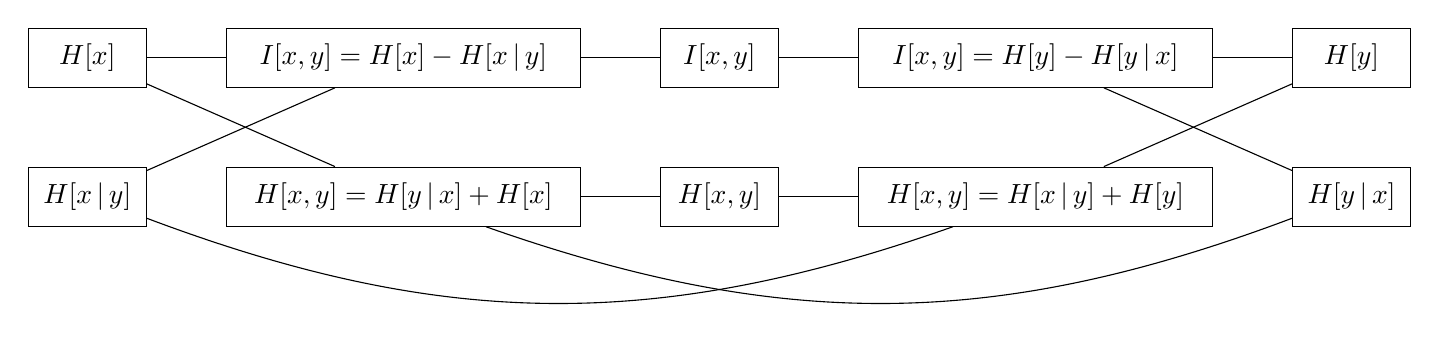
\begin{tikzpicture}[
							quantity/.style = {
								draw,
								rectangle,
								minimum width = 1.5cm,
								minimum height = 0.75cm,
							},
							relation/.style = {
								draw,
								rectangle,
								minimum width = 4.5cm,
								minimum height = 0.75cm,
							}
						]
					\node [quantity] (iXY) {\( I[x, y] \)};
					\node [quantity, below = 1 of iXY] (hXY) {\( H[x, y] \)};

					\node [relation, left = 1 of iXY] (iFromHx) {\( I[x, y] = H[x] - H[x \given y] \)};
					\node [relation, right = 1 of iXY] (iFromHy) {\( I[x, y] = H[y] - H[y \given x] \)};
					\node [relation, left = 1 of hXY] (hXYFromX) {\( H[x, y] = H[y \given x] + H[x] \)};
					\node [relation, right = 1 of hXY] (hXYFromY) {\( H[x, y] = H[x \given y] + H[y] \)};

					\node [quantity, left = 1 of iFromHx] (hX) {\( H[x] \)};
					\node [quantity, right = 1 of iFromHy] (hY) {\( H[y] \)};
					\node [quantity, left = 1 of hXYFromX] (hXgY) {\( H[x \given y] \)};
					\node [quantity, right = 1 of hXYFromY] (hYgX) {\( H[y \given x] \)};

					\draw (iFromHx) to (iXY);
					\draw (iFromHx) to (hX);
					\draw (iFromHx) to (hXgY);

					\draw (iFromHy) to (iXY);
					\draw (iFromHy) to (hY);
					\draw (iFromHy) to (hYgX);

					\draw (hXYFromX) to (hXY);
					\draw (hXYFromX) to (hX);
					\draw (hXYFromX) to[bend right = 20] (hYgX);

					\draw (hXYFromY) to (hXY);
					\draw (hXYFromY) to (hY);
					\draw (hXYFromY) to[bend left = 20] (hXgY);
				\end{tikzpicture}
				\caption{Relations between the entropies and mutual information of two random variables, \(x\) and \(y\).}
				\label{fig:1-39-entropy}
			\end{figure}
		% end

		\subsection{Arithmetic and Geometric Mean  \onestar}
			By applying the logarithm and Jensen's inequality to the geometric mean,
			\begin{equation}
				\log(\, \prod_{i = 1}^{n} x_i \!)^{\!1/n}
					= \frac{1}{n} \log \prod_{i = 1}^{n} x_i
					= \frac{1}{n} \sum_{i = 1}^{n} \log x_i
					\leq \log( \frac{1}{n} \sum_{i = 1}^{n} x_i ),
			\end{equation}
			it can be seen that the logarithm of the arithmetic mean is never less than the logarithm of the geometric mean. By applying the exponential on both sides of the inequality, it follows that also the arithmetic mean itself is never less than the geometric mean.

			\qedeot
		% end

		\subsection{Mutual Information  \onestar}
			The relation \( I[\vec{x}, \vec{y}] = H[\vec{x}] - H[\vec{x} \given \vec{y}] \) can be shown straightforwardly by splitting the integral:
			\begin{align}
				I[\vec{x}, \vec{y}]
					&= -\!\iint\! p(\vec{x}, \vec{y}) \, \log \frac{p(\vec{x}) \, p(\vec{y})}{p(\vec{x}, \vec{y})} \dd{\vec{x}} \dd{\vec{y}} \\
					&= -\!\iint\! p(\vec{x}, \vec{y}) \, \log p(\vec{x}) \dd{\vec{x}} \dd{\vec{y}} + \iint\! p(\vec{x}, \vec{y}) \, \log \frac{p(\vec{x}, \vec{y})}{p(\vec{y})} \dd{\vec{x}} \dd{\vec{y}} \\
					&= -\!\iint\! p(\vec{x}, \vec{y}) \, \log p(\vec{x}) \dd{\vec{x}} \dd{\vec{y}} + \iint\! p(\vec{x}, \vec{y}) \, \log p(\vec{x} \given \vec{y}) \dd{\vec{x}} \dd{\vec{y}} \\
					&= H[\vec{x}] - H[\vec{x} \given \vec{y}]
			\end{align}
			This concludes the proof. Showing \( I[\vec{x}, \vec{y}] = H[\vec{y}] - H[\vec{y} \given \vec{x}] \) is analogous.

			\qedeot
		% end
	% end
\end{document}





















